\subsection{Mirrors Re-coating}

As seen in Fig.~\ref{fig:optics}, each segment is composed of four optical surfaces: one elliptical mirror,
one hyperbolic mirror, one cylindrical mirror and the Winston cone.

Several mirrors's reflectivity was measured and show significant degradation from the original
desired reflectivty of $90\%$ in the visible spectrum, see Fig.~\ref{fig:reflectivityBefore}.

A refurbishment of the mirrors was crucial to enhance the detector response to the pion emitted Cherenkov light.
Due to the material, assembly and dimension of the different type of mirrors, two different techniques were applied.

\begin{figure}[h]
\centering
	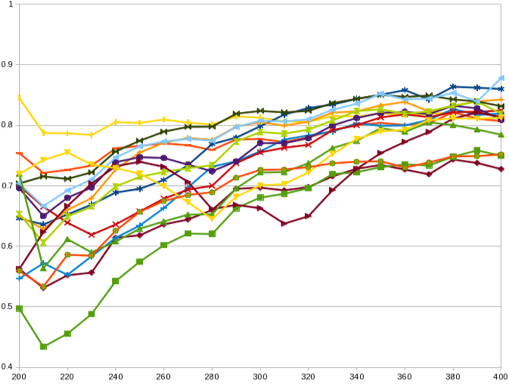
\includegraphics[width=1.0\columnwidth,keepaspectratio]{img/mirrorsReflectivityBefore.png}
	\caption{Average number of reflections calculated from simulations studies.}
	\label{fig:reflectivityBefore}
\end{figure}


\subsubsection{Re-coating of Cylindical mirrors}

The cylindrical mirrors range from 6 to 12 inches in length. Each mirror is made by a single piece of aluminum or plastic.
Due to the small size, it can fit in most vacuum chambers used to coat mirrors by evaporation of aluminum with magnesium fluoride
($AlMg_2$). After successful testing a re-coating of $AlMg_2$ onto the existing substrate, the work of recoating 216 cylindrical mirrors
was awared to ECI~\cite{ECI}. See Fig.~\ref{fig:reflectivityAfter} for typical reflectivity values after recoating.


\subsubsection{Re-coating of Elliptical and Hyperbolic mirrors}

The elliptical and hyperbolic mirrors are composed by a kevlar support structure with a lexan substrate. The mounting hardware
material, that allowed for pitch, roll and yaw alignment of the mirrors, included wood and aluminum that was glued to the support structure.

Several companies attempted to re-coat these mirrors but failed due to the outgassing of the various material. Furthermore many of the mirrors
are $> 50$'' in length, longer than most vacuum chambers. In summary, the $AlMg_2$ could not be re-deposited directly on the mirrors.

A different approach consisted of coating thin (25 microns) lexan strips and glue the strips on the mirror's substrate. While promising, this
presented the challenge of protecting the coated lexan strip from shipping and handling and from the gluing procedure to the mirrors.

A working chain was setup to:

\begin{enumerate}
	\item coating the lexan strip
	\item protection with a film
	\item shipping
	\item gluing to mirrors
	\item testing reflectivity
\end{enumerate}

An example of unwrapping the film off the lexan strip is shown in Fig.~\ref{fig:filmOnStrip}. Several companies produced various test. In the end the
job was awarded to ECI~\cite{ECI}. The typical reflectivity of the refurbished mirrors is shown in Fig.~\ref{fig:reflectivityAfter}.

\begin{figure}[h]
\centering
	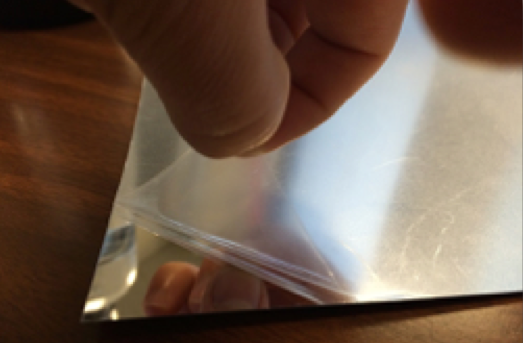
\includegraphics[width=0.98\columnwidth,keepaspectratio]{img/filmOnStrip.png}
	\caption{For the elliptical and hyperbolic mirrors lexan strips were coated with $AlMg_2$ then glued on top of the mirrors. The photo shows
            the process of removign the protecting film from one such strip.}
	\label{fig:filmOnStrip}
\end{figure}


\subsubsection{Elliptical Mirrors Gaps}

The segment with long elliptical mirrors presented several gaps between them, some a few cm long. To make sure that no light is lost in these gaps,
additional 120 micron thick lexan extension coated with $AlMg_2$ were glued to cover the gaps. The strips were manufactured by ECI~\cite{ECI}.



\subsubsection{Mirrors re-coating summary and results}

All 216 cylindrical mirrors were re-coated on the existing surface. All 216 elliptical and 216 hyperbolic mirrors were refusrbished using lexan strip
coated with $AlMg_2$ glued on the substrate. The different sizes of the mirrors were accounted for using different width of the lexan strips, see
summary table~\ref{tab:strips}.


\begin{table}[h]
	\begin{center}
		\begin{tabular}{| l | c |}
			\hline \hline
			Quantity  & Description \\
			\hline
			190       & 9" x 36" x 0.010” coated sheet    \\
			150       & 10" x 36" x 0.010” coated sheet   \\
			6         & 10" x 36" x 0.010” coated sheet   \\
			\hline \hline
		\end{tabular}
	\end{center}
	\caption{Summary of material used for the elliptical and hyperbolic mirrors.}\label{tab:strips}
\end{table}

\begin{figure}[h]
\centering
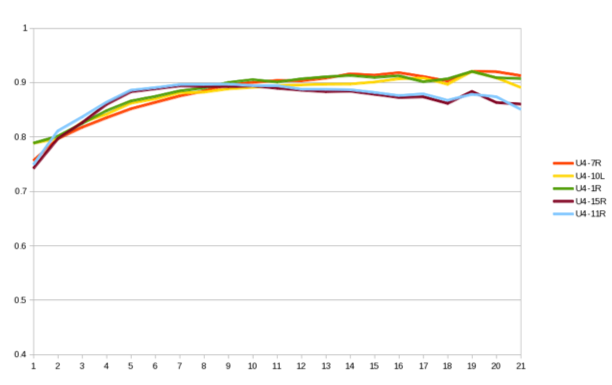
\includegraphics[width=0.95\columnwidth,keepaspectratio]{img/mirrorsReflectivityAfter.png}
\caption{Typical mirror reflectivity measure after re-coating the mirrors or glueing the lexan strips. Note the very high value of reflectivity
in the UV region, where most of the Cherenkov light is produced. In the visible spectrum, the reflectivity is about $\sim 90\%$.}
\label{fig:reflectivityAfter}
\end{figure}



In Fig.~\ref{fig:reflectivityAfter} a typical spectrum of reflectivity that applies to all cylindrical, elliptical and hyperbolic mirrors is shown.
The re-coated mirrors shows a $\sim 90\%$ reflectivity in the visible spectrum and an exceptional $\sim 80\%$
reflectivity in the UV spectrum,


\subsection{Mirrors Alignment}

A new procedure was developed to align the mirrors that takes advantage of their focusing capabilities. The elliptical mirrors focal points are 1. the target
(origin of the lab coordinate system)
and 2. a point behind the hyperbolic mirror. The focal points if the hyperbolic mirrors are 1. a point near the focal point of the elliptical mirrors and
2. above the face of the PMTs.

The mathematical shape of the mirrors has been build in the geant4 simulation, see Fig.~\ref{fig:alignmentSimulation}. When a laser line is directed at the mirror,
it is focused on the hyperbolic focal point, then directed at the PMT.

\begin{figure}[h]
\centering
	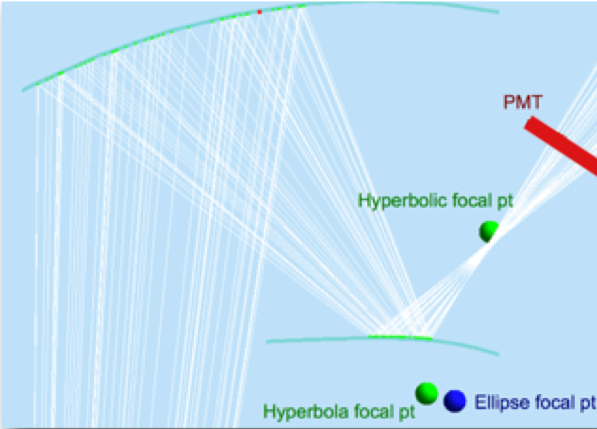
\includegraphics[width=1.0\columnwidth, keepaspectratio]{img/mirrorAlignmentSimulationZoomed.png}
	\caption{The simulation of a laser line (white tracks are photons) originating from the target and directed at the elliptical mirrors. The photons are directed
		      at the second ellipse focal point, and the hyperbolic mirror reflects them on its focal point. This picture illustrate the procedure used to align the mirrors.}
	\label{fig:alignmentSimulation}
\end{figure}

The laser setup for the mirror alignment is shown in Fig.~\ref{fig:laserAlignment}. A 3 mW, $635 nm$ laser was placed, relative to the detector,
in the lab center of coordinate system. The position was accurate at the 0.5 mm level. The laser was spread through two cylindrical lenses onto a laser line and shone
onto each elliptical mirror. Both the elliptical and hyperbolic mirrors were rotated to focus the light onto the face of the PMT.

\begin{figure}[h]
\centering
	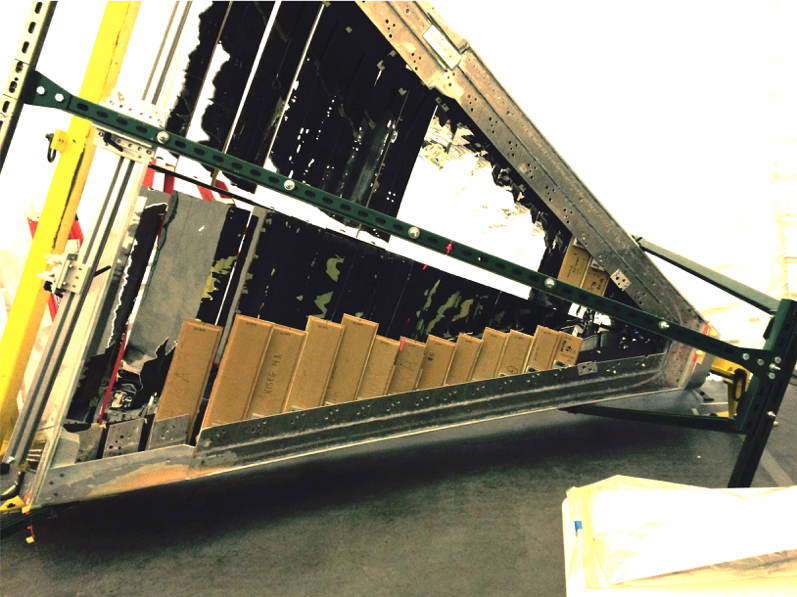
\includegraphics[width=0.95\columnwidth, keepaspectratio]{img/laserAlignment1.png}
	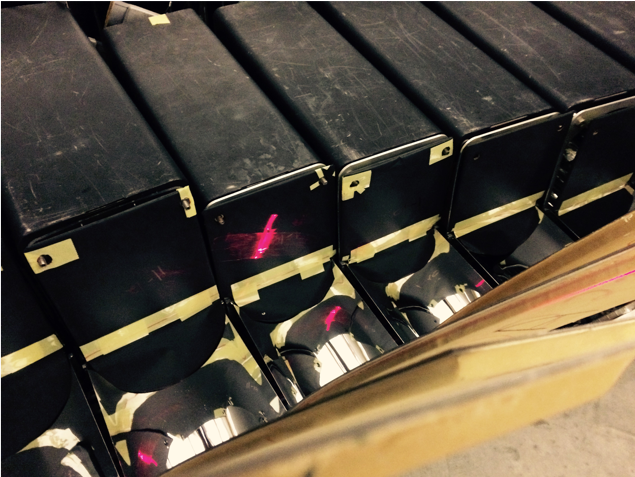
\includegraphics[width=0.95\columnwidth, keepaspectratio]{img/laserAlignment2.png}
\caption{The laser aligment setup. Top: the laser was placed, relative to the detector, in the lab coordinate system. The laser line was shined on each elliptical mirror.
         Bottom: zoomed in view of the laser line focused on the center of the PMT after the mirrors were aligned.}
	\label{fig:laserAlignment}
\end{figure}

